\documentclass[12pt, twoside]{article}
\documentclass[12pt, twoside]{article}
\usepackage[letterpaper, margin=1in, headsep=0.2in]{geometry}
\setlength{\headheight}{0.6in}
%\usepackage[english]{babel}
\usepackage[utf8]{inputenc}
\usepackage{microtype}
\usepackage{amsmath}
\usepackage{amssymb}
%\usepackage{amsfonts}
\usepackage{siunitx} %units in math. eg 20\milli\meter
\usepackage{yhmath} % for arcs, overparenth command
\usepackage{tikz} %graphics
\usetikzlibrary{quotes, angles}
\usepackage{graphicx} %consider setting \graphicspath{{images/}}
\usepackage{parskip} %no paragraph indent
\usepackage{enumitem}
\usepackage{multicol}
\usepackage{venndiagram}

\usepackage{fancyhdr}
\pagestyle{fancy}
\fancyhf{}
\renewcommand{\headrulewidth}{0pt} % disable the underline of the header
\raggedbottom
\hfuzz=2mm %suppresses overfull box warnings

\usepackage{hyperref}
\usepackage{siunitx}

\title{IB Mathematics}
\author{Chris Huson}
\date{May 2024}

%\fancyhead[LE]{\thepage}
\fancyhead[RO]{\thepage \\ Name: \hspace{1cm} \,\\}
\fancyhead[LO]{BECA/Huson/Algebra II: Regents Prep \\* 6 May 2024}

\begin{document}

\subsubsection*{Practice Regents problems \#7}
AII-F.BF.2: Write arithmetic and geometric sequences both recursively and with an explicit formula, use them to model situations, and translate between the two forms.

\begin{enumerate}
\item Given the sequence $a$: 32, 24, 18, 13.5, $\ldots$
\begin{enumerate}[itemsep=4cm]
    \item State whether the sequence is arithmetic, geometric, or neither. Justify your answer.
    \item Write a recursive formula for $a$.
    \item Write an explicit formula for the sequence.
    \item Find the sum of the first three terms the sequence.
\end{enumerate}

\item Express the fraction $\displaystyle \frac{3x^{\frac{5}{2}}}{(27x^3)^{\frac{2}{3}}}$ in simplest radical form. \vspace{3cm}

\newpage
AII-F.LE.2: Construct a linear or exponential function symbolically given: a graph, a description of the relationship, or two input-output pairs (include reading these from a table).

\item The area, in square meters, of a pond covered by an algae bloom decreases exponentially after a treatment is applied.
\begin{enumerate}[itemsep=1cm]
    \item Fill out the table, giving the area covered by the algae in square meters days after the treatment is applied.
    \begin{center}
    \begin{tabular}{|p{1cm}|p{1cm}|p{1cm}|p{1cm}|p{1cm}|p{1cm}|}
        \hline
        Days & 0 & 1 & 2 & 3 & 4 \\
        \hline
        Area & 150 & & 50 & & \\[0.25cm]
        \hline
    \end{tabular}
    \end{center}
    \item Another pond has an algae bloom that is also decreasing exponentially. The
    area of this bloom in square meters is given by the function $B(d)=120 \times 3^{-\frac{d}{3}}$, where $d$ is days since the first measurement of the bloom. 
    \begin{center}
        \begin{tikzpicture}[x=1cm, y=0.05cm, xscale=2.5]
            \draw [thin, color=lightgray, xstep=0.5cm,ystep=0.5cm] (0,0) grid (4,160);
            \draw [thick, ->] (0,0) -- (+4.3,0) node [below]{$d$};
            \draw [thick, ->] (0,0) -- (0,165) node [left]{$Area$};        
            \foreach \x in {0,1,...,4}
                \draw (\x cm,5pt) -- (\x cm,-5pt) node[below] {$\x$};
            \foreach \y in {0,20,...,160}
                \draw[shift={(0,\y)}] (2pt,0pt)--(-2pt,0pt) node[left]{$\y$};
            %\draw [thick, ->, smooth,domain=0.:4.1] plot(\x,{120*(0.333^(\x/3))});
            %\fill (0,90) ellipse [x radius=1pt, y radius=2.5pt]  node [right] {$(0,32)$};
            %\fill (2,30) ellipse [x radius=1pt, y radius=2.5pt] node [above right] {$(1.5,4)$};
        \end{tikzpicture}
        \end{center}
    \item Which of the two algae blooms was larger initially? Which is decreasing more quickly? Explain how you know.
\end{enumerate}


\end{enumerate}
\end{document}